\documentclass[11pt, oneside]{article}
\usepackage{titling, hyperref, geometry, amsmath, amssymb, algorithm, graphicx, textcomp, subcaption, cancel}
\usepackage[noend]{algpseudocode}
\usepackage[cache=false]{minted}
\geometry{a4paper}

\hypersetup{
    colorlinks=true,
    urlcolor=cyan
}

\newcommand{\emphasis}[1]{\textbf{\textit{#1}}}
\graphicspath{{./images/}}

\title{Range Minimum Query with Fischer-Heun (Abridged)}
\author{Stephen Huan\\ Edited by: Udbhav Muthakana}

\begin{document}
\maketitle

\section{Definition}

The \emphasis{Range Minimum Query} (RMQ) problem is defined as follows: \\
Given an array \( A \) with length \( n \) and two indexes \( i, j \mid i \leq j \),
find the smallest element between \( i \) and \( j \) (inclusive on both ends).

\section{Algorithms}
\subsection{Dynamic Programming}

There are only \( \Theta(n^2) \) possible queries because \( i \) can take on \( n \) possible values
and \( j \geq i \).

If we precompute every possible query, then we can answer them in \( O(1) \). Naïvely computing the table
with an \( O(n) \) scan for each query will take \( O(n^3) \) for all the queries.
Instead, we can use dynamic programming. Consider the base case of \( i = j \);
the minimum is the only element in the range. Now consider a range of length \( l \) starting
at \( i \), given the minima for all ranges of length \( l - 1 \).
The answer would just be the minimum between the range starting at \( i \) with a length of \( l - 1 \),
and the range starting at \( i + 1 \).

\begin{figure}[h!]
\centering
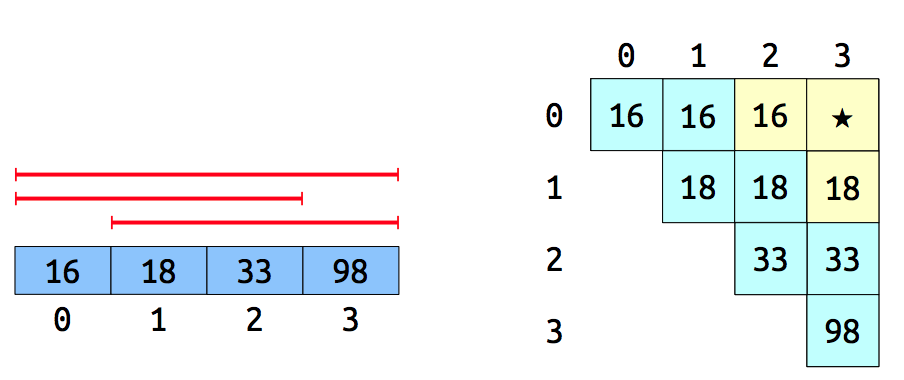
\includegraphics[scale=0.25]{dp}
\caption{Decomposing a range into smaller ranges and the DP table.}
\end{figure}

Since there are \( O(n^2) \) states and transitions between states are calculated in \( O(1) \),
this is an \( O(n^2) \) DP, yielding an \( \langle O(n^2), O(1) \rangle \) RMQ structure. We now have two solutions:
\( \langle O(1), O(n) \rangle \) with no preprocessing and \( \langle O(n^2), O(1) \rangle \) with full preprocessing.

\subsection{Sparse Tables}

Instead of precomputing all \( O(n^2) \) possible ranges, it suffices to only compute a certain subset of ranges
and still maintain constant time query. The key observation is that any range can be broken down into subranges
with lengths that are powers of two.

\begin{figure}[h!]
\centering
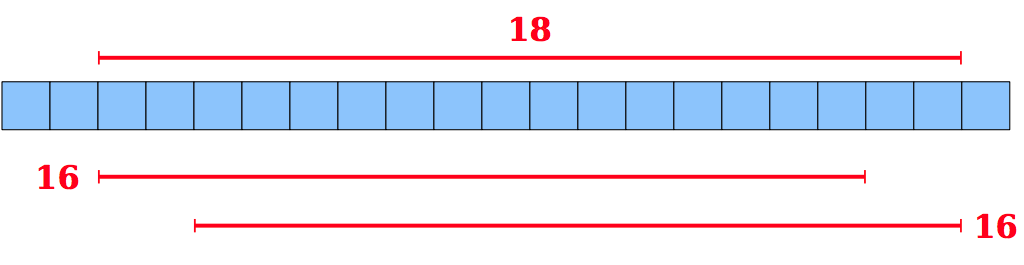
\includegraphics[scale=0.25]{sparse_decomp}
\caption{Breaking up a range into powers of two}
\end{figure}

For each starting index \( i \), precompute the minimum in the ranges with lengths
\( 1, 2, 4, \dots 2^l \), where \( l \) is at most \( \log n \). In order to answer a query,
find the largest \( k \) such that \( 2^k \leq j - i + 1 \).
The simplest method is to compute \( \lfloor \log_2{(j - i + 1)} \rfloor \).

Then, think of the range \( [i, j] \) as the union between the ranges \( [i, i + 2^k] \) and \( [j - 2^k, j] \).
Each range has already been precomputed, so the query is \( O(1) \).

In order to precompute the \( O(n \log n) \) ranges, we use dynamic programming again.
The base case of \( i = j \) is again to choose the only element in the range. Consider a range of length \( l \) starting
at \( i \), given the minima for all ranges of length \( \frac{l}{2} \). The answer would just be
the range starting at \( i \) with length \( \frac{l}{2} \) and the range starting at \( i + \frac{l}{2} \).

Overall, \emphasis{sparse tables} yield an \( \langle O(n \log n), O(1) \rangle \) solution to RMQ.

\subsection{Block Decomposition}

Consider splitting the array into \( \frac{n}{b} \) blocks, where each block
has a size of \( b \). Compute the minimum value in each block.

\begin{figure}[h!]
\centering
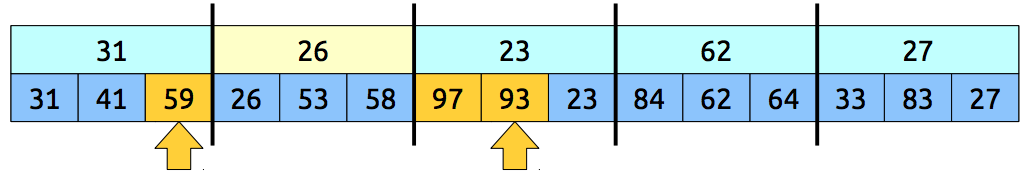
\includegraphics[scale=0.25]{block}
\caption{Array with block size \( b = 3 \)}
\end{figure}

Suppose \( i \) and \( j \) are in different blocks with blocks in between them
(the cases where \( i \) and \( j \) are in the same block, or they are in different but adjacent blocks
are trivial). To answer a RMQ query, scan from \( i \)'s position to the end of its block,
\( j \)'s position to the beginning of its block, and instead of scanning each element in between
\( i \) and \( j \), use the precomputed block minima.

The preprocessing time is \( O(b) \) to find the minimum in each block, times
\( \frac{n}{b} \) blocks for \( O(n) \). The total query cost is \( O(b + \frac{n}{b}) \),
optimal if \( b = \sqrt{n} \), yielding a \( \langle O(n), O(\sqrt{n}) \rangle \) solution to RMQ.
This technique is actually called ``Square root bucketing'' and has been covered in past SCT lectures.

\subsection{Hybrids}

Instead of naïvely scanning inside blocks and over the block minima, we can build another RMQ
structure on top! The algorithm is then as follows:
\begin{itemize}
  \item Split the input array into blocks of size \( b \).
  \item Form a smaller array of block minima.
  \item Create a ``summary'' RMQ structure over the block minima array.
  \item Create ``block'' RMQ structures for each block.
  \item Merge the results together for queries.
\end{itemize}

\begin{figure}[h!]
\centering
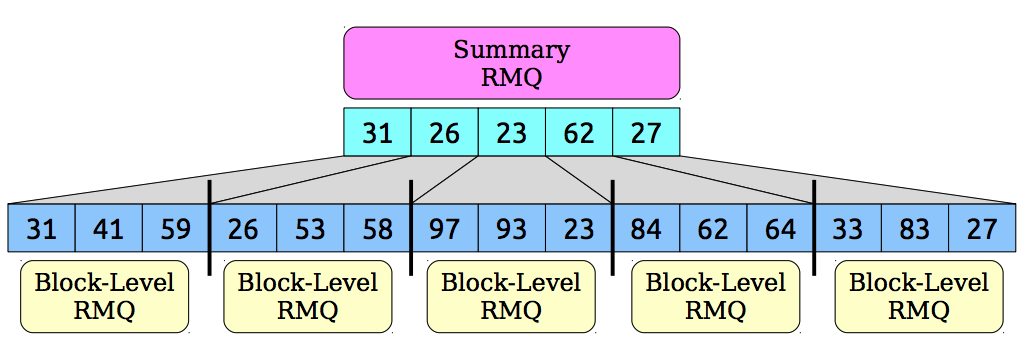
\includegraphics[scale=0.25]{summary}
\caption{Top level view of the overall RMQ structure}
\end{figure}

In order to analyze the running time of this new hybrid structure, let
\( \langle f(n), g(n) \rangle \) be the time for the block minima and
\( \langle p(n), q(n) \rangle \) be the time for each block.
The construction time is then \( O(n + f(\frac{n}{b}) + \frac{n}{b} p(b)) \),
and the query time is \( O(g(\frac{n}{b}) + q(b)) \).

\subsection{Fischer-Heun}

\subsubsection{Block Types}
Suppose we have the arrays \( B_1 = [1, 3, 2, 4] \) and \( B_2 = [10, 30, 20, 40] \).
Although the arrays are different, the answer to any RMQ query is going to be the same,
since they have a similar \emphasis{type} (which we'll represent as \( B_1 \sim B_2 \)).
If we find that two blocks have the same type, we can reuse the RMQ structure of one
for the other without computing it again. We'll also use the aforementioned sparse table
for the top and the fully precomputed solution for the blocks.
The precomputation time is then
\[ O(n + \frac{n}{b} \log n + (\text{\# of distinct blocks}) b^2) \]

We now have two questions:
\begin{enumerate}
  \item How do we tell if \( B_1 \sim B_2 \)?
  \item How many different types are there?
\end{enumerate}

\subsubsection{Detecting Block Types}
The approach stems from the observation that if \( B_1 \sim B_2 \), they must have minimum elements
at the same position. If they didn't, a range query over the length of the array would yield different answers.
This property must also hold recusively on the subarrays to the left and to the right of the min.
These observations lead us to Cartesian trees.

\begin{figure}[h!]
\centering
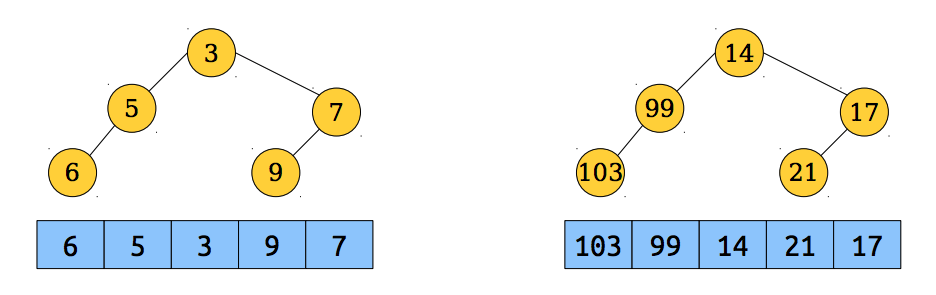
\includegraphics[scale=0.25]{cartesian}
\caption{Cartesian trees}
\end{figure}

A \emphasis{Cartesian tree} is a binary tree where an inorder traversal yields the original array and is a min-heap.
The following theorem follows: \( B_1 \sim B_2 \) iff \( B_1 \) and \( B_2 \)
have isomorphic, i.e. same shape Cartesian trees.
In order to check whether two arrays have isomorphic Cartesian trees, we need to be able to
build a Cartesian tree quickly.
In order to maintain the fact that an inorder traversal yields the original array,
new nodes must be added as right children with the previous elements to their left.
In order to maintain the fact that the tree is a min-heap,
we can only add a new node as a child of nodes it's greater than.
These two observations form the following algorithm:
\begin{itemize}
  \item Keep a stack of ``active'' nodes.
  \item To insert a new node:
    \begin{itemize}
      \item While the stack is not empty and the top node has a value greater than the new node:
      \begin{itemize}
        \item Pop nodes off the stack
      \end{itemize}
      \item Make the parent of the new node the top of the stack, or null
      if the stack is empty (the new node is now the root).
      \item Make the left child of the new node the last node that was popped off the stack,
      null if nothing was popped off.
      \item Add the new node to the stack.
    \end{itemize}
\end{itemize}

This algorithm runs in \( \Theta(n) \) and does at most \( 2n \) operations.

In order to check whether two trees are isomorphic, notice that
the resulting Cartesian tree is determined by the sequence of pushes and pops from the stack.
If we call a push ``1'' and a pop ``0'', then we have a binary number we'll call the
\emphasis{Cartesian tree number} with length at most \( 2n \). In order to compare two arrays,
we'll compare the two Cartesian tree numbers.
This approach answers our first question of determining whether \( B_1 \sim B_2 \), but
we still need to determine how many possible unique blocks there are. If our number is at most \( 2b \) bits long,
where \( b \) is the size of each block, then there are at most \(2^{2b} = 4^b \) possible numbers.

\subsection{The Final Algorithm}

\begin{figure}[h]
\centering
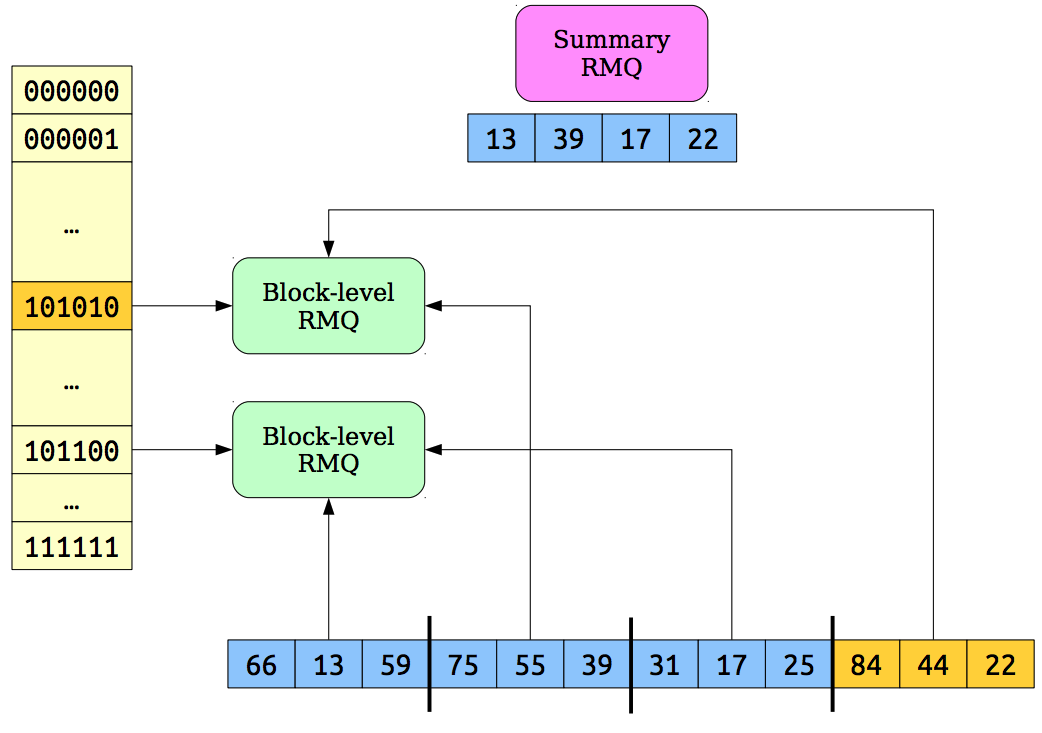
\includegraphics[scale=0.25]{final}
\caption{The final RMQ structure}
\end{figure}

Recall that we used a sparse table on the summary array with full precomputation on each block,
yielding a query time of \( O(1) \). Our precomputation time is:
\[ O(n + \frac{n}{b} \log n + (\text{\# of distinct blocks}) b^2) \]
and with our Cartesian tree observation, the number of distinct blocks is at most \( 4^b \).
\[ O(n + \frac{n}{b} \log n + 4^b b^2) \]
In order to pick \( b \), note that \( 4^b \) grows exponentially if \( b > \log n \), and \( \frac{n}{b} \log n \)
will be greater than \( n \) if \( b < \log n \). Thus, we should pick \( b = k \log_4 n \) where \( k \) is some constant.

Going back to the expression we had for the preprocessing time:
\[ O(n + n + n^k (k \log_4 n)^2) \]

The standard pick is \( k = \frac{1}{2} \), but that seems mostly arbitrary.

To conclude, we now have a \emphasis{Fischer-Heun structure} that solves RMQ
in an asymptotically optimal \( \langle O(n), O(1) \rangle \).

\begin{itemize}
  \item Set \( b = k \log_4 n = \frac{1}{2} k \log_2 n \) where \( k = \frac{1}{2} \).
  \item Split the array into blocks of size \( b \) and calculate the minimum for each block.
  \item Build a sparse table on that minima array.
  \item Build fully preprocessed RMQ structures on each block, avoiding recomputing the
  same RMQ structure for blocks with the same Cartesian tree number.
  \item Answer queries using the standard hybrid approach.
\end{itemize}

\section{Sample Problems}

\begin{enumerate}
  \item \href{https://www.spoj.com/problems/RMQSQ/}{SPOJ RMQSQ}: Direct application of RMQ.

  \item \href{http://www.usaco.org/index.php?page=viewproblem2&cpid=576}{USACO Max Flow}
  or any problem involving Lowest Common Ancestor (LCA).
  LCA can be converted into RMQ in linear time and vice versa - the method is to
  perform an Euler tour on the tree. An Euler tour is essentially a combination of a
  preorder traversal and a postorder traversal that yields a list of nodes.
  If a node has children, we add it to the list and then recursively
  DFS on its children. After the recursive DFS call, we add the node to the list again.
  The LCA between two nodes in the graph must appear between the two nodes in this array.
  Other nodes not on the path between the two nodes may also appear between them,
  but they are guaranteed to have greater heights than the LCA.

  Some implementation details: I maintain a dictionary mapping a node to its first
  occurence in the array, the array itself, which contains the height of each node,
  and an inverse array mapping a position in the array to the node which it represents. \\
  The LCA between two nodes \( u, v \) is then inverse[RMQ(array, indexes[u], indexes[v])].

  \item \href{https://www.spoj.com/problems/BEADS/}{SPOJ BEADS}, \href{https://www.spoj.com/problems/LPS/}{SPOJ LPS},
  \href{https://leetcode.com/problems/longest-palindromic-substring/}{Leetcode LPS}, \href{https://leetcode.com/problems/palindromic-substrings/}{Leetcode palindromic-substrings}, etc.

  The \emphasis{L}ongest \emphasis{C}ommon \emphasis{P}refix (LCP) is
  the length of the longest common prefix between two strings.
  For example, the LCP between ``abcd'' and ``abef'' is 2.
  The \emphasis{LCP array} is then the LCP value between adjacent suffixes in the suffix array
  (the suffix array stores all of the suffixes of a given string sorted lexicographically).

  However, our LCP array only stores the LCP value for adjacent suffixes.
  How do we generalize to the LCP between any two suffixes?

  The observation is that the LCP value between two nonadjacent suffixes
  is the minimum LCP value between them in the LCP array.
  To see why this is true, notice that LCP decreases monotonically moving away from a suffix.
  Since the suffix array is sorted lexicographically, suffixes with a larger LCP
  value must be closer than suffixes with a smaller LCP value to a particular suffix.
  Call the LCP value \( h \) and the minimum LCP value between the two suffixes \( m \).
  \( h \leq m \) because of monotonicity.
  Also, \( h \geq m \) because a range minimum of \( m \) implies that there exists a prefix of length \( m \)
  common to all the suffixes between two suffixes, thus the LCP is at least \( m \).
  If \( m \leq h \leq m \), then \( h = m \).

  Thus, we can construct the Fischer-Heun RMQ structure on the LCP array.
  Then, the LCP between two suffixes \( i \) and \( j \) is lcp[rmq(lcp, i, j - 1)] assuming \( i \leq j \)
  which is an \( O(1) \) query. This allows us to solve a variety of string problems.

  \item RMQ can simulate a sliding window/monotonic queue.

\end{enumerate}

\end{document}
